\documentclass[a4paper,12pt]{article}

\usepackage[utf8]{inputenc}
\usepackage[T1]{fontenc}
\usepackage[brazil]{babel}
\usepackage{graphicx}
\usepackage{xcolor}
\usepackage{tcolorbox}
\usepackage{geometry}
\usepackage{tikz}
\usetikzlibrary{positioning, shapes.multipart}
\geometry{margin=2.5cm}
 
\definecolor{meuazul}{RGB}{0, 79, 151}

\begin{document} 

\begin{center}
    
\includegraphics[width=3cm]{logo.png} \\
    \vspace{0.5cm}
    \textbf{\large Engenharia da Qualidade e Confiabilidade} \\
    \textbf{Atividade Prática: Planning Poker}
\end{center}

\vspace{1cm}

\begin{tcolorbox}[colback=meuazul!5, colframe=meuazul, title=\textbf{HU004: Registro de Ordenhas}]
    
    \textbf{Título:} Controle de Produção Diária por Animal
    
    \vspace{0.3cm}
    \textbf{Descrição (História de Usuário):} \\
    Como \textbf{Funcionário / Ordenhador}, \\
    quero \textbf{registrar a quantidade de leite coletada de cada vaca}, \\
    para \textbf{monitorar a produtividade do rebanho e identificar variações anormais}.
    
    \vspace{0.3cm}
    \textbf{Valor de Negócio:} \\
    Essencial para o cálculo de produtividade e detecção precoce de doenças (ex: mastite).
    
    \vspace{0.3cm}
    \textbf{Prioridade:} Crítica
    
\end{tcolorbox}

\vspace{0.5cm}

\section*{Story Points e Protótipos de Tela}
\begin{enumerate}
    \item \textbf{Lançar Ordenha:} Selecionar Vaca, Data/Hora, Litros e Observação.
    \begin{itemize}
        \item \textit{Explicação:} Registro principal de produção. Deve permitir vincular a vaca e o funcionário responsável.
        \begin{center} 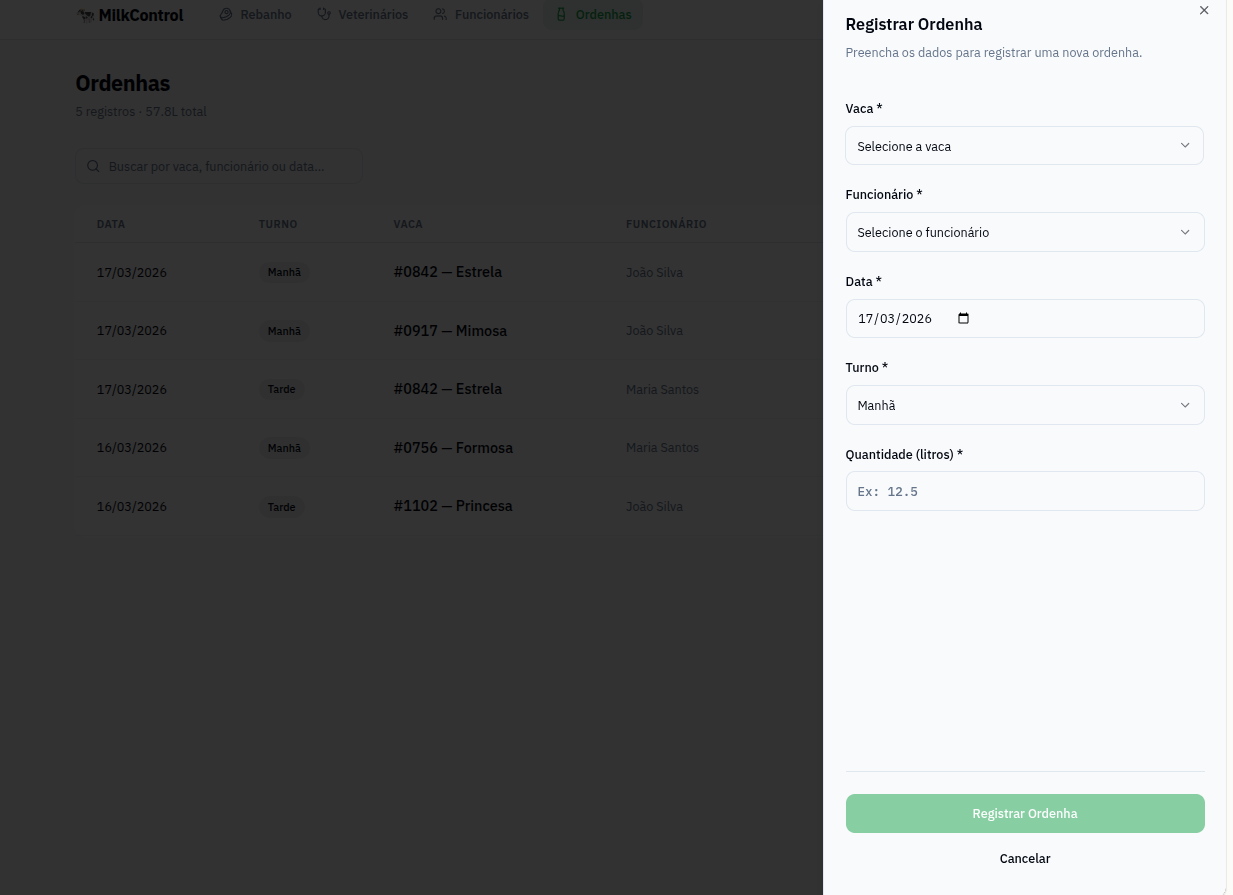
\includegraphics[width=0.7\textwidth]{create_ordenha.png} \end{center}
    \end{itemize}

    \item \textbf{Visualizar Histórico:} Ver produção de uma vaca ou data específica.
    \begin{itemize}
        \item \textit{Explicação:} Listagem cronológica das ordenhas realizadas.
        \begin{center} 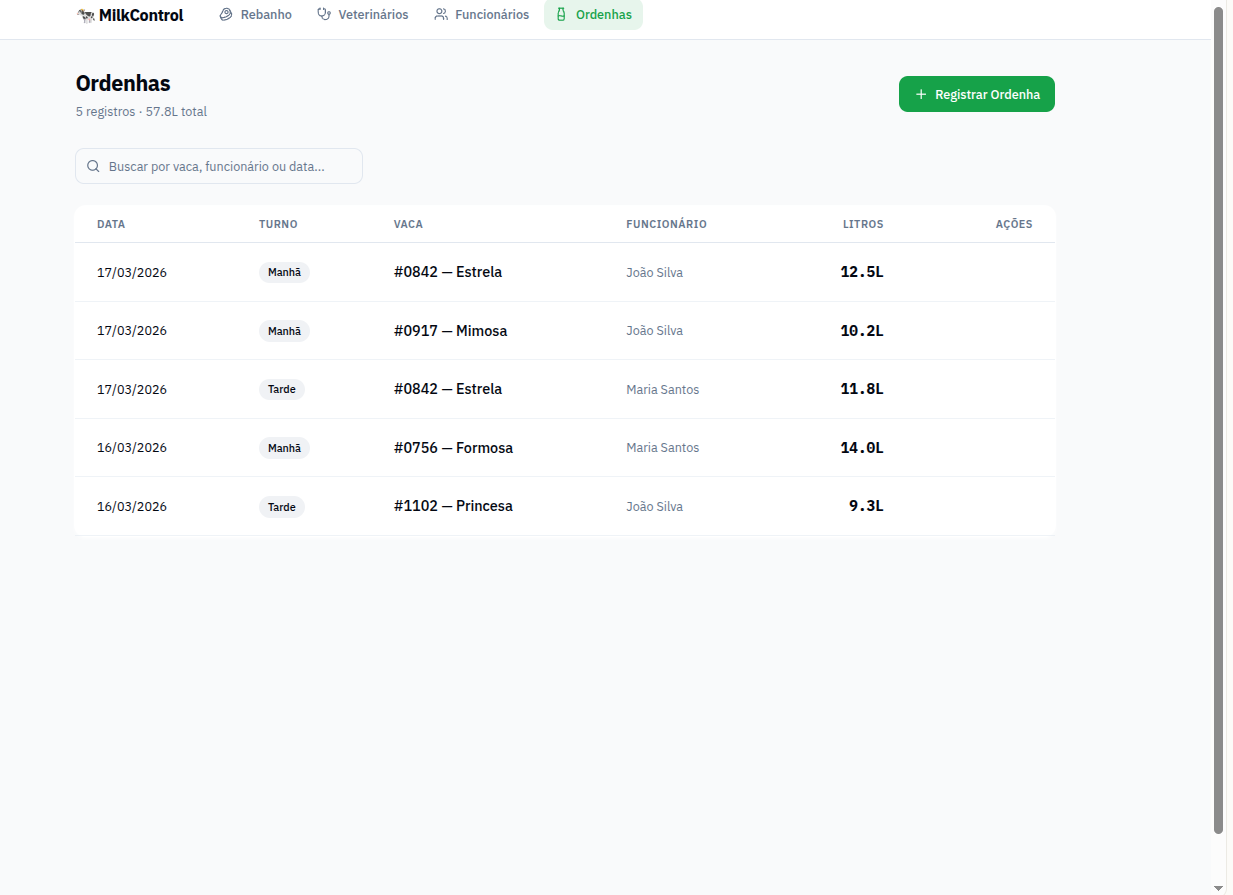
\includegraphics[width=0.7\textwidth]{show_ordenha.png} \end{center}
    \end{itemize}

    \item \textbf{Editar Lançamento:} Corrigir erro de digitação nos litros ou hora.
    \begin{itemize}
        \item \textit{Explicação:} Ajustes em registros feitos incorretamente nas últimas horas.
    \end{itemize}

    \item \textbf{Cancelar Lançamento:} Estornar registro indevido.
    \begin{itemize}
        \item \textit{Explicação:} Remoção de registros duplicados ou errôneos.
        \begin{center} 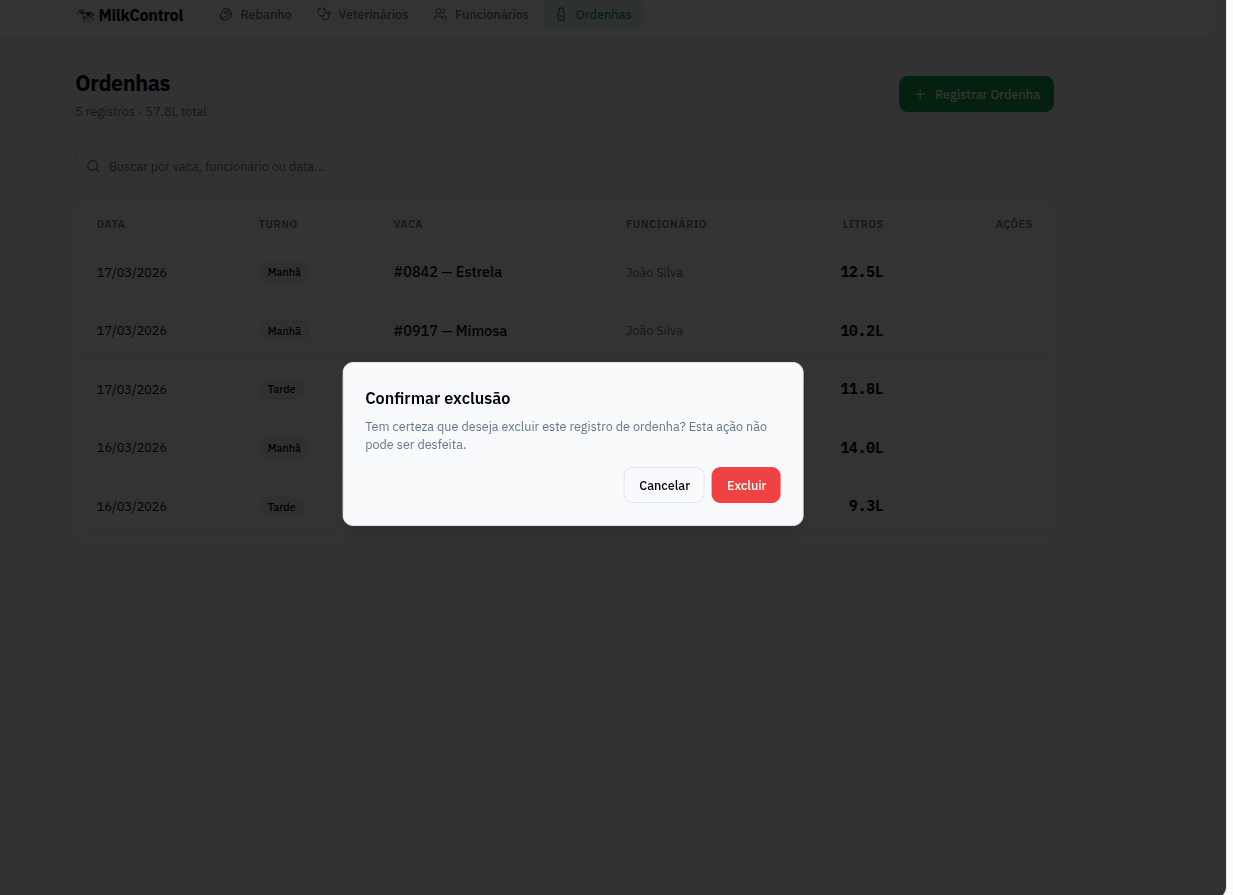
\includegraphics[width=0.7\textwidth]{delete_ordenha.png} \end{center}
    \end{itemize}
\end{enumerate}

\vspace{0.5cm}

\section*{Modelo de Dados (Diagrama de Classes)}

\begin{center}
\begin{tikzpicture}[
    node distance=2cm,
    classBox/.style={
        draw=meuazul,
        thick,
        fill=white,
        minimum width=3.5cm,
        rectangle split,
        rectangle split parts=3,
        align=left,
        rounded corners=2pt
    }
]

% Classe Ordenha
\node[classBox] (Ordenha) {
    \textbf{Ordenha}
    \nodepart{second}
    - id: Integer \{PK\} \\
    - dataHora: DateTime \\
    - litros: Float
    \nodepart{third}
    + salvar()
};

% Classe Vaca
\node[classBox, left=3cm of Ordenha] (Vaca) {
    \textbf{Vaca}
    \nodepart{second}
    - brinco: String \{PK\}
    \nodepart{third}
};

% Classe Funcionario
\node[classBox, right=3cm of Ordenha] (Func) {
    \textbf{Funcionario}
    \nodepart{second}
    - cpf: String \{PK\}
    \nodepart{third}
};

% Associações
\draw[thick, meuazul] (Vaca) -- (Ordenha) node[pos=0, above right] {1} node[pos=1, above left] {*};
\draw[thick, meuazul] (Func) -- (Ordenha) node[pos=0, above left] {1} node[pos=1, above right] {*};

\end{tikzpicture}
\end{center}

\vspace{0.5cm}

\section*{Atividade: Estimativa com Planning Poker}

Cada grupo deverá estimar o esforço das funcionalidades utilizando \textbf{Story Points} (Fibonacci):

\begin{center}
\textbf{0, 1, 2, 3, 5, 8, 13, 21}
\end{center}

\vspace{1cm}

\begin{center}
    \rule{0.5\textwidth}{0.4pt} \\
    \small UniRV - Engenharia de Software
\end{center}

\end{document}
